\documentclass[a4paper,twocolumn,10pt]{article}
\usepackage{usenix,epsfig,endnotes,listings,graphicx,hyperref}
\begin{document}

%don't want date printed
\date{}

%make title bold and 14 pt font (Latex default is non-bold, 16 pt)
\title{\Large \bf Continuous Integration of The FreeBSD Project}

\author{
{\rm Li-Wen Hsu}\\
{\rm The FreeBSD Project}\\
{\rm \href{mailto:lwhsu@FreeBSD.org}{lwhsu@FreeBSD.org}}
}

\maketitle

% Use the following at camera-ready time to suppress page numbers.
% Comment it out when you first submit the paper for review.
\thispagestyle{empty}

\subsection*{Abstract}
The FreeBSD project's continuous integration project started in the late 2013.
We use Jenkins automation server to build our continuous integration system.
It monitors the svn repository for new commits and triggers a new build of it.
In each build, the build machine compiles the latest code, creates disk image
and creates a virtual machine to run test suite. In the meantime, we collect
the compiler warnings and perform some further checks like clang analyzer. All
these information are published to the developers and users to improve the
quality of the FreeBSD project. In this paper, we describe the details of the
system implementation.

\section{Introduction}

The term of continuous integration (CI) is first used by Grady Booch in 1991,
then Extreme programming (XP) extends the concept of CI and suggests to
integrate as many times as possible per day. Now, CI is an important and common
practice of software engineering. The benefits of CI are developers can know
the conflicts and bugs earlier. This reduces the cost for resolving them later.
Also, the status of the project is clearer and it is easier to estimate
progress.

There are many software designed for various CI need, among them, the most
popular one is Jenkins, an open source automation server written in Java,
created by Kohsuke Kawaguchi. We use Jenkins as the main component, along with
some other daemons like Pure-FTPd, to build FreeBSD project's CI system.

We describe the history of FreeBSD's CI work, how we trigger build from changes
in version control system, do tests and publish results in the rest of this
paper.

\section{Automatic Build and History of CI work in FreeBSD}

Dag-Erling Smørgrav created the first pubic CI system for the FreeBSD project:
\url{http://tinderbox.FreeBSD.org}, this can be traced back in the mail archive in
March 2002. It is believed the first continuous integration service of the
FreeBSD project. Tinderbox is an open source project, codes are available at
svn://svn.freebsd.org/base/user/des/tinderbox .  Documents can be found in
FreeBSD doc project and wiki. Unfortunately this service stopped in September
or October 2014, nevertheless, here are many scripts from this project derived
or inspiring the successive projects.

In late 2013, Craig Rodrigues founded jenkins-admin@FreeBSD.org with several
developers. The main duty of jenkins-admin is maintaining the jenkins
instance in FreeBSD cluster, \url{https://jenkins.FreeBSD.org}. Which is an
independent successor of tinderbox.FreeBSD.org. We configure it monitors the
FreeBSD src and doc repositories, and triggers a new build when there is new
commit in each supported branch. We created the first "build-and-test pipeline"
for the FreeBSD project. In each build triggered by a change in repository,
after compiling successes, we create a virtual machine disk image with the
latest binaries, and spawn a new virtual machine to run tests. The test results
are collected and stored by jenkins server.

The highlight features of jenkins.FreeBSD.org are:

\begin{itemize}
\item Periodically build for head, stable-11, stable-10 and stable-9
\item Architectures built against: amd64, i386, sparc64 and arm64
\item Build FreeBSD with GCC, using amd64-xtoolchain-gcc
\item Experimental Jenkins 2 "pipeline as code"
\end{itemize}

Shortly, jenkins.FreeBSD.org become a significant role in the FreeBSD
development.

In 2016, with the hardwares sponsored by the FreeBSD foundation, we created
\url{https://ci.FreeBSD.org}, an experimental site for testing new ideas. We
still leverage Jenkins because it has proven useful on jenkins.FreeBSD.org. We
implemented:

\begin{itemize}
\item Artifact server
\item Job template
\end{itemize}

Having a centralized artifact server enables people retrieving the files
generated from each stage of a build, for reproducing issues for debugging
purpose, or doing further tests. The details about job template are in "open
configurations" section. Another experiment in this system is we are trying to
make the build pipeline more fine-grained, and introduced more build types. For
example, we not only created virtual machine disk image specialized for tests,
but try to produce the distribution files and virtual machine disk images same
as official release from release engineering provided. Also, we build LINT
kernel for more test coverage.

The naming conversion of the build jobs is:
$FreeBSD-{branch}-{target\_arch}-{stage}$. For each supported branch and
architecture, there are several jobs in a full pipeline.  Take head branch and
amd64 architecture for example:

\begin{itemize}
\item FreeBSD-head-amd64-build\\
  Build the world and kernel from scratch and creates distribution files.
\item FreeBSD-head-amd64-LINT\\
  Build the LINT kernel
\item FreeBSD-head-amd64-images\\
  Build virtual machine disk images from distribution files with the same configuration of official release
\item FreeBSD-head-amd64-testvm\\
  Build virtual machine disk image from distribution files and test files and package are pre-installed.
\item FreeBSD-head-amd64-test\\
  Run the image from "testvm" stage in a new created virtual machine.
\end{itemize}

\begin{figure*}
\includegraphics[width=\textwidth]{pipeline.eps}
\caption{head-amd64 pipeline}
\label{pipeline}
\end{figure*}

Their relationship is shown in ~\ref{pipeline}

The codes are available at \url{https://github.com/lwhsu/freebsd-ci} and
\url{https://github.com/lwhsu/jjb-freebsd-ci}, merging back to the main
freebsd-ci repository or even svn.freebsd.org is proceeding.

\section{Self Tests}

In 2013 Rui Paulo created the \path{/usr/tests} hierarchy, with the Kyua test
framework by Julio Merino. These tests can be performed by command:
\begin{lstlisting}
cd /usr/tests && kyua test
\end{lstlisting}
As of January 2017, we have 6023 tests for head branch on amd64 architecture.

As previous section mentioned, we build virtual machine disk images with the
required files and packages for running tests. We pre-install the kyua package
and put a script which runs kyua commands, and generates the test reports after
all tests are executed. Finally it issues shutdown command. After the disk
image ready, for amd64 and i386 architecture, we launch a bhyve virtual
machine, with a expect script for starting running tests in, and also for
catching timeout in case.

After the testing virtual machine stopped, we extracted the test results from
the disk image, and put to the workspace where jenkins will send back to the
master for accounting. The script to create test virtual machine image is
\path{scripts/build/build-test_image.sh}, and the main script for executing
tests in virtual machines and extracting results is
\path{scripts/test/run-tests.sh}.

\section{Access to Results}

We configure Kyua to generate results as JUnit XML format, which is natively
supported by Jenkins, and many other tools. Jenkins default plugins take
outputs from the builds, make it a friendly accessible web interface at
\url{https://<job-url>/<build-number>/testReport} (fig. ~\ref{test-result},
~\ref{failed-result}), and maintains a historical data (fig.
\ref{test-result-trend}). This helps us tracking the software quality trending.

\begin{figure*}
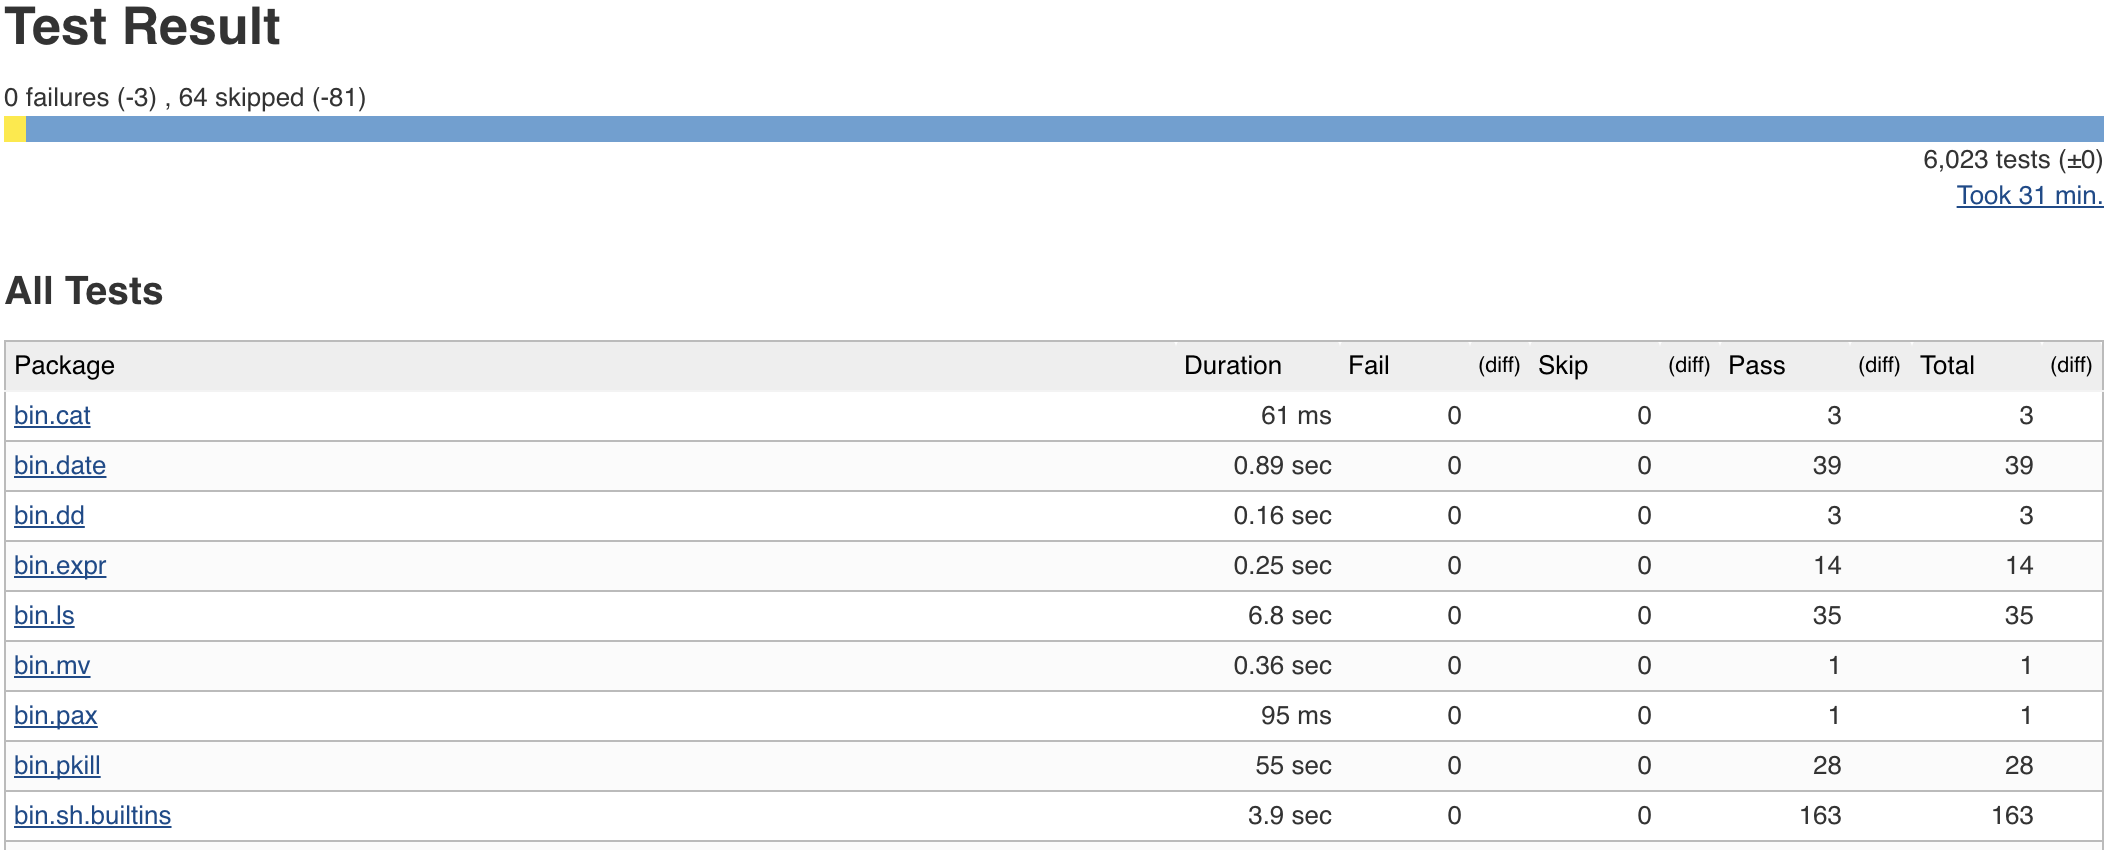
\includegraphics[width=\textwidth]{test-result.png}
\caption{Test result from a test job}
\label{test-result}
\end{figure*}

\begin{figure*}
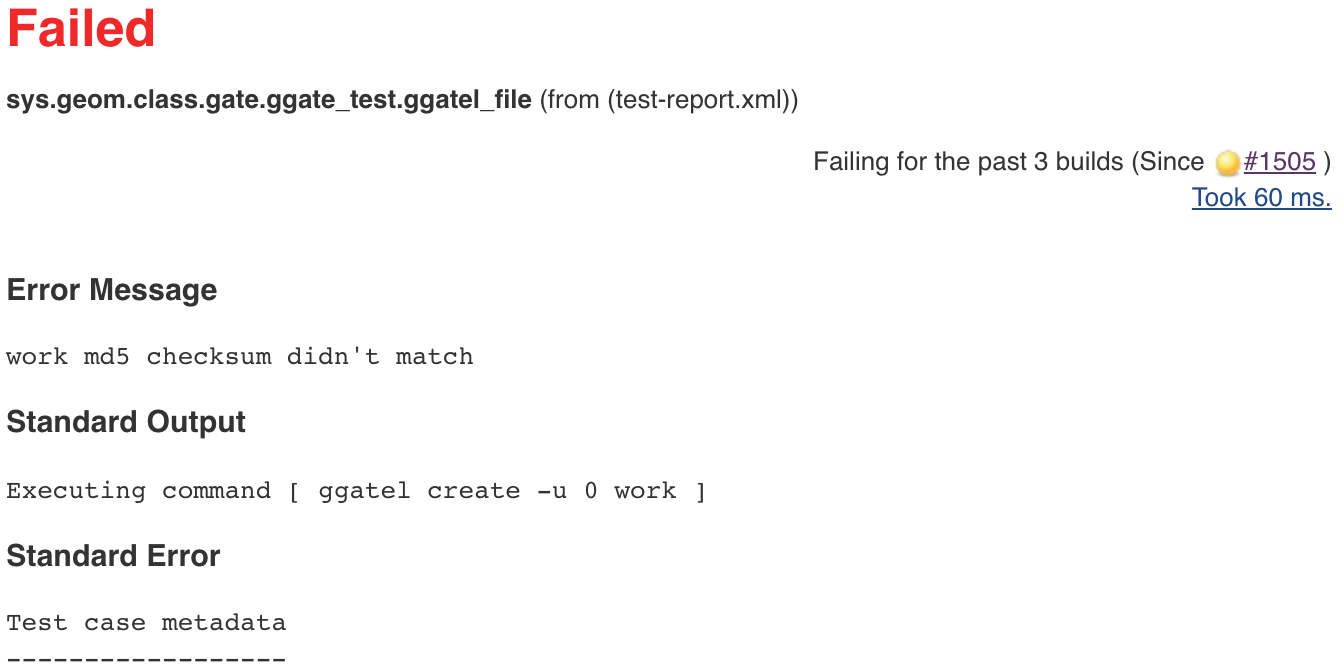
\includegraphics[width=\textwidth]{failed-result.png}
\caption{Failed test case display}
\label{failed-result}
\end{figure*}

\begin{figure*}
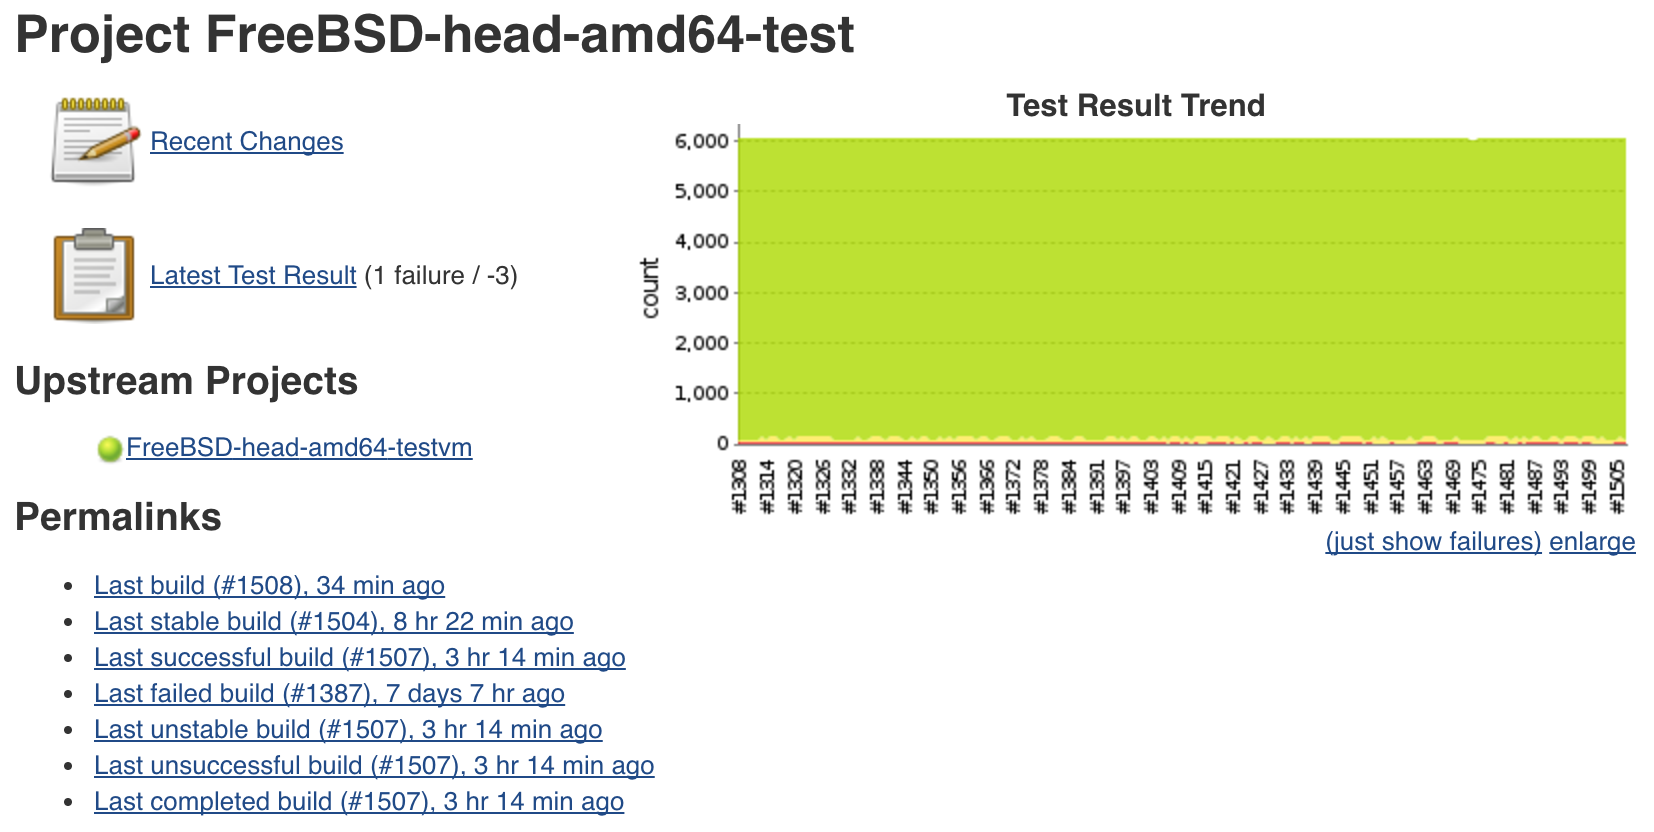
\includegraphics[width=\textwidth]{test-result-trend.png}
\caption{Test result trend}
\label{test-result-trend}
\end{figure*}

The artifact.ci.FreeBSD.org is newly introduced in ci.FreeBSD.org, we upload
the artifacts created in each stage of a build pipeline. We Add FTP over TLS
feature in "Publish Over FTP Plugin", in the end of each stage, Jenkins uploads
created files through FTPES, there is only one root directory  "snapshots" in
artifact.ci.FreeBSD.org, and the directory layout of it is:
\path{{branch}/{svn_revision}/{target}/{target_arch}}, for example,
\path{head/r303226/amd64/amd64} . This layout is compatible with the official
download site. We hope that in the future these snapshot artifacts can also be
included and be more easily accessed by users.

Currently we have these artifacts for each pipeline:

\begin{itemize}
\item *.txz
  \begin{itemize}
  \item From *-build jobs
  \item Distribution files just like what on \url{https://download.FreeBSD.org}
  \end{itemize}
\item disk.img.xz
  \begin{itemize}
  \item From *-images jobs
  \item Virtual machine disk image file, installed from above *.txz files
  \end{itemize}
\item disk-test.img.xz
  \begin{itemize}
  \item From *-testvm jobs
  \item Virtual machine disk image file, with test script and test case
  \end{itemize}
\end{itemize}

All files are publicly available at \url{http://artifact.ci.freebsd.org}.

\section{Open Configurations}
It is very important to make public can setup a highly identical instance of a
public service, and security is also need to be considered. In the past,
Jenkins job can only be edited on web interface, which is not easy to tracking
the changes and reproduce. Users who has no administrative permission cannot
see exactly configurations. Jenkins 2.0's "pipeline as code" is a very
promising to solve this problem. On jenkins.FreeBSD.org, we have tested it for
the jobs which build head and stable-10 branch. The source code is available at
\url{https://github.com/freebsd/freebsd-ci/blob/master/scripts/build/build-test.groovy}.
However, currently not all the required Jenkins plugins of ci.FreeBSD.org
supports this. We will look into this again and may switch it later.

We use an approach used by other project for a long time, Jenkins job builder,
which converts YAML files to Jenkins XML configurations. And manipulate Jenkins
instance via web service. With Jenkins job builder, the configuration of
Jenkins is trackable and reproducible, and we can separate security credentials
to other storage.

While working with other developers, we found the fact that not everyone knows
(and has to know) how to configure Jenkins. So adding new build jobs requires
Jenkins administrators configure and test build scripts by hand. This is a
bottleneck of the development. We also found that most of the build jobs are
just having different build scripts, other parts of the configurations such as
repository URL and notification settings are the same. It inspired us to create
a "job template" for similar jobs. A typical job contains following steps:

\begin{enumerate}
\item Environment setup
  \begin{enumerate}
  \item Check out latest source code
  \item Setup needed version of FreeBSD
  \item Install required packages
  \end{enumerate}
\item Execute specified build script for that job
\item Environment cleanup
\end{enumerate}

The respective job definition (of Jenkins job builder) is very simple
(listing \ref{jjb-job-def}):

\begin{lstlisting}[captionpos=b,caption=Job definition,label=jjb-job-def]
- job:
    name: FreeBSD-head-scan_build
    scm:
      - FreeBSD-src-head
    builders:
      - checkout-scripts
      - setup-jail
      - execute-in-jail
    publishers:
      - clean-jail
    wrappers:
      - timestamps
\end{lstlisting}

And we use jail to ensure the freshness of the build environment, and we can
install "sudo" program inside jail, with full privileges granted, for maximum
the things user can do for testing. As a result, "build-in-jail script sets" is
created, they are currently developed at
\url{https://github.com/lwhsu/freebsd-ci/tree/jjb/scripts/jail}. It's first job
is simplify environment setup and job execution, we have three scripts for each
builder and publishers in definition of jenkins job builder:

\begin{itemize}
\item setup.sh\\
  setup-jail builder, setup a jail jail and install require packages
\item execute.sh\\
  execute-in-jail builder, execute build scripts from user
\item clean.sh\\
  clean-jail publisher, clean the used jail to release resource
\end{itemize}

A typical job configuration contains three files:

\begin{itemize}
\item build.sh\\
  Main build script, which is executed by execue.sh in the jail
\item jail.conf\\
  Jail environment configuration: version, arch, etc.
\item pkg-list\\
  Package needs to be installed (from pkg.FreeBSD.org)
\end{itemize}

With these, adding a new job is much simplified. Submitter can just test their
tested build script (build.sh), with some job definitions (jail.conf,
pkg-list), and other configuration files, for example, src.conf or make.conf.
Then jenkins-admin merges scripts to freebsd-ci/jobs/<job name>/, and
jenkins-admin creates a new job entry in jenkins job builder, push the new
configuration to the Jenkins server. Everything is done. Our Jenkins server
will execute it around the clock.

For example, FreeBSD-head-arm64-build contains files as listing \ref{job-conf}:

\begin{lstlisting}[captionpos=b,caption=Job configurations,label=job-conf]
(jail.conf)
TARGET=amd64
TARGET_ARCH=amd64
WITH_32BIT=0
OSRELEASE=10.3-RELEASE

(pkg-list)
aarch64-binutils

(build.sh)
#!/bin/sh
env \
  JFLAG=${BUILDER_JFLAG} \
  TARGET=arm64 \
  TARGET_ARCH=aarch64 \
  sh -x freebsd-ci/scripts/build/build-world-kernel.sh
\end{lstlisting}

We also add a "quarantine mode" of "build-in-jail script sets", just specify
"QUARANTINE=1" in jail.conf, the the internet connection is removed after jail
environment is setup, and resource is also strictly limited, such as execution
time.

The other ci.FreeBSD.org setup can be found at
\url{https://wiki.freebsd.org/Jenkins/Setup}.

\section{Other Integrations}

The best feature of Jenkins is its features can be extended by many plugins, we
selected several plugins which considered useful for us and integrated into our
system.

\subsection{Notification}

Make sure related developers can know the latest project status is very
important. We use both Email and IRC notifications. The status for sending out
notifications are:

\begin{itemize}
\item Build failed
\item Build unstable (compile successfully, but some test cases failed)
\item Build back to stable
\end{itemize}

And for notification email, we attach following information:
\begin{itemize}
\item Changes since last build (who \& what)
\item Tail of the console output
\item What are the test cases failed
\item Related URLs
\end{itemize}

Email notification is considered a "double-edged sword", once we send out too
many mails and people will consider them as spam. If nobody reads the
notification mails and takes action, it is totally no use. So use carefully
created a pre-send script with "Email-ext plugin", for filter out the internal
errors of the jenkins cluster, to reduce false alert. The script is available
at:
\url{https://github.com/freebsd/freebsd-ci/blob/master/scripts/email-ext/pre-send.groovy}
.

\subsection{Code Review System}

The FreeBSD project owns a code review system at \url{https://reviews.FreeBSD.org},
which is setup with Phabricator, and jenkins has a "Phabricator Differential
Plugin" plugin. It currently supports only git, we patched it to support
subversion, and are also preparing to upstream it.

On ci.FreeBSD.org, we have two jobs:

\begin{itemize}
\item FreeBSD-head-amd64-build-phabric
\item FreeBSD-doc-head-igor-phabric
\end{itemize}

They are using "quarantine mode" of the "build-in-jail script sets", and are
triggered when a new patch is uploaded to reviews.FreeBSD.org (fig.
~\ref{build-patch}).

\begin{figure*}
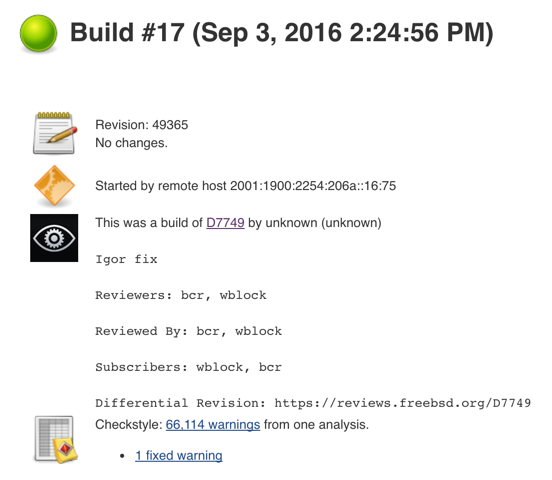
\includegraphics{build-patch.png}
\caption{Build triggerd by a patch}
\label{build-patch}
\end{figure*}

And reports the build result back to reviews.FreeBSD.org (fig.
~\ref{patch-build-result}).

\begin{figure*}
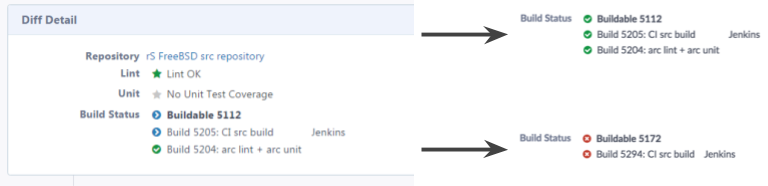
\includegraphics[width=\textwidth]{patch-build-result.png}
\caption{Rsult of a build triggerd by a patch}
\label{patch-build-result}
\end{figure*}

\subsection{Clang Static Analyzer}

We created a "clang clang-build" job with Clang Static Analyzer, and leveraged
the "bsd.clang-analyzed.mk" from NetBSD, simple build the whole world and
kernel with:

\begin{lstlisting}
make analyze \
CLANG_ANALYZE_OUTPUT_DIR=clangScanBuildReports \
CLANG_ANALYZE_OUTPUT=html
\end{lstlisting}

command, then the result being taken cared by "Clang Scan-Build Plugin", which
generates good web interface and history tracking (fig.
\ref{scan-build-result}, \ref{scan-build-path}, \ref{clang-scan-build-trend})

\begin{figure*}
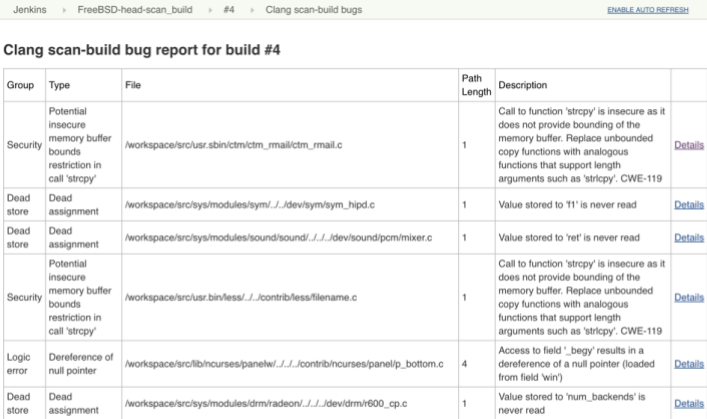
\includegraphics[width=\textwidth]{scan-build-result.png}
\caption{Clang scan-build result}
\label{scan-build-result}
\end{figure*}

\begin{figure*}
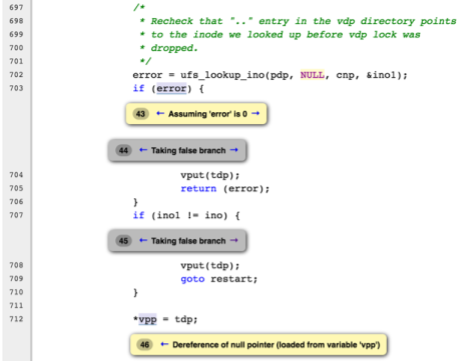
\includegraphics[width=\textwidth]{scan-build-path.png}
\caption{Clang scan-build result explanation}
\label{scan-build-path}
\end{figure*}

\begin{figure*}
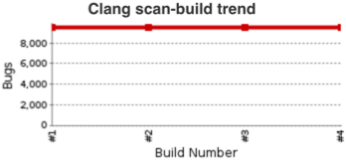
\includegraphics{clang-scan-build-trend.png}
\caption{Clang scan-build trend}
\label{clang-scan-build-trend}
\end{figure*}

\subsection{Igor and Checkstyle}

For document build, we use igor by Warren Block, and Checkstyle for checking
the style of document XML. We worked with Warren and added a new option (-X) to
igor, to output checkstyle XML. The respective job is FreeBSD-doc-head-igor.
"Checkstyle Plugin" of Jenkins also provides good web interface and history
tracking. (fig \ref{checkstyle-result}, \ref{checkstyle-compare},
\ref{checkstyle-trend})

\begin{figure*}
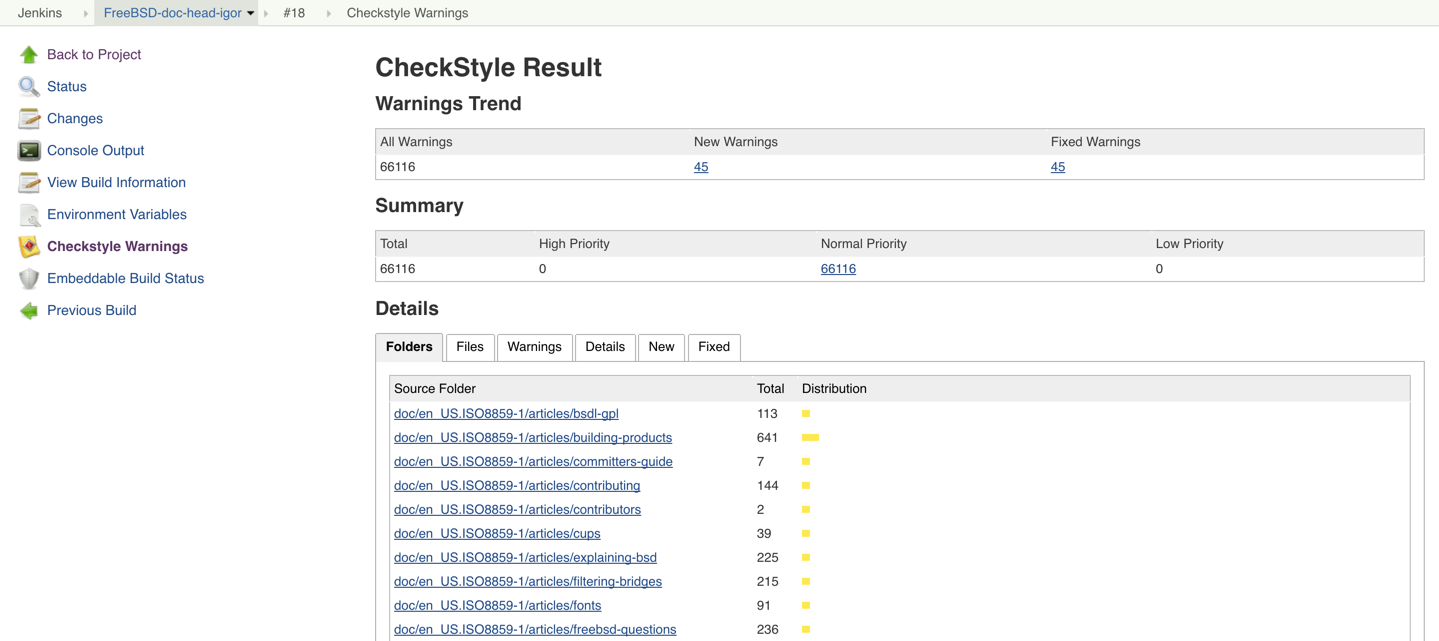
\includegraphics[width=\textwidth]{checkstyle-result.png}
\caption{Igor + Checksytle - result}
\label{checkstyle-result}
\end{figure*}

\begin{figure*}
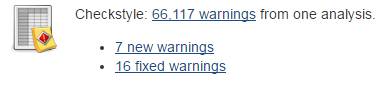
\includegraphics{checkstyle-compare.png}
\caption{Igor + Checkstyle - compare with previous build}
\label{checkstyle-compare}
\end{figure*}

\begin{figure*}
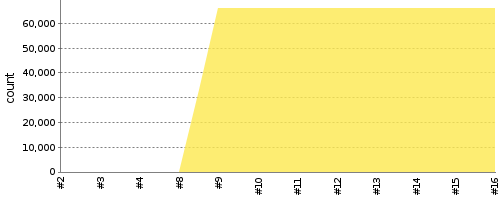
\includegraphics{checkstyle-trend.png}
\caption{Igor + Checkstyle - trend}
\label{checkstyle-trend}
\end{figure*}

\subsection{Compiler Warnings}

We also collect compiler warnings with "compiler warning" plugin. For showing
the trend of compiler warnings and this pushes developers produce higher
quality code. (fig. \ref{compiler-result}, \ref{compiler-trend})

\begin{figure*}
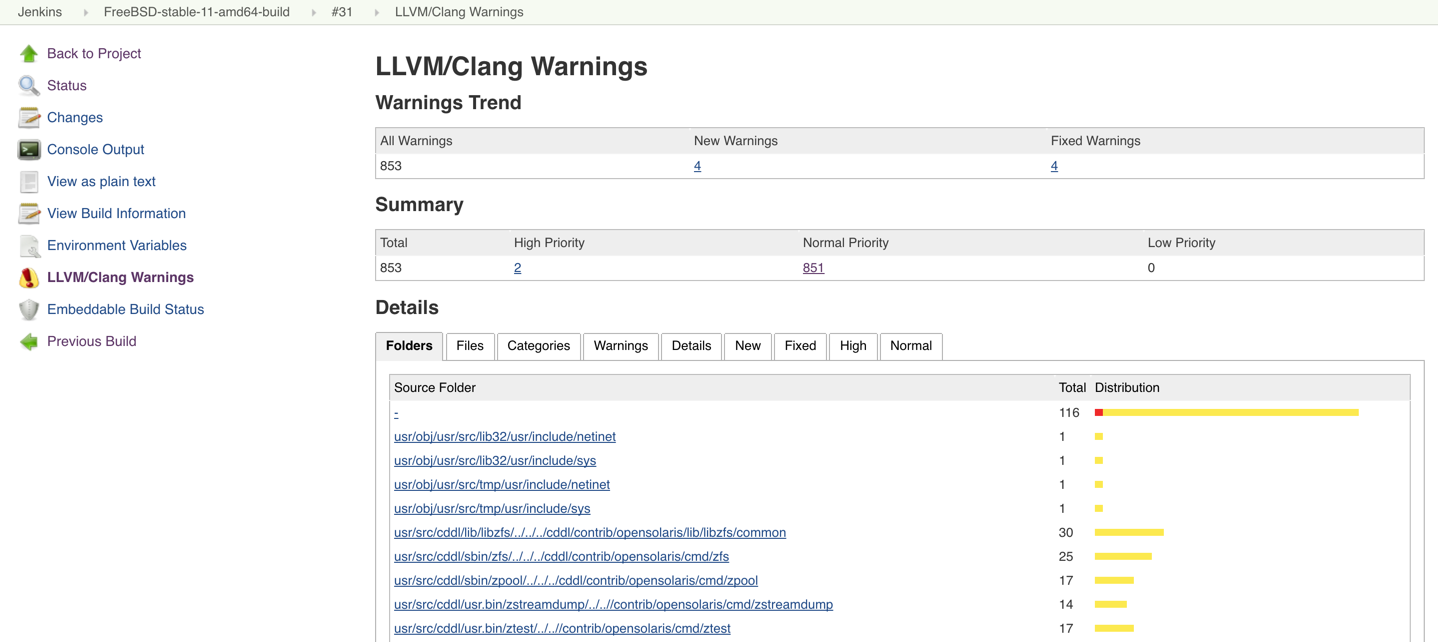
\includegraphics[width=\textwidth]{compiler-result.png}
\caption{Compiler Warnings - result}
\label{compiler-result}
\end{figure*}

\begin{figure*}
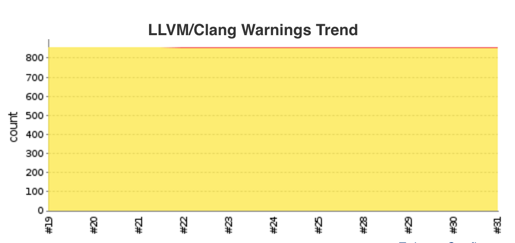
\includegraphics{compiler-trend.png}
\caption{Compiler Warnings - trend}
\label{compiler-trend}
\end{figure*}

\subsection{Build Status Badge}

We provide build status badge for embedding in external web pages. For example,
on \url{https://wiki.FreeBSD.org/arm64} , we have badge as fig.
~\ref{build-status-badge}

\begin{figure*}
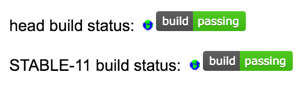
\includegraphics{build-status-badge.png}
\caption{Build satus badge}
\label{build-status-badge}
\end{figure*}

To show the latest status of each branch. The badge URLs are:
\begin{itemize}
\item \url{https://<job-url>/badge/icon}
\item \url{https://<job url>/lastCompletedBuild/badge/icon}
\end{itemize}

\subsection{Others}

We also use some other plugins for improving the interface and helping the
maintenance task:

\begin{itemize}
\item SCM Sync configuration
  \begin{itemize}
  \item Use post-commit hook to notify administrators
  \end{itemize}
\item SafeRestart
  \begin{itemize}
  \item Schedule restart jenkins when all current jobs complete
  \item Save and resume the build queue
  \end{itemize}
\item Green balls
  \begin{itemize}
  \item To replace blue status ball with green ones, to fulfill the convention
        for most culture.
  \end{itemize}
\end{itemize}

\section{Conclusion}

In this paper, we described about the history and how we setup the latest CI
system of the FreeBSD project.  CI does help the development of the FreeBSD
project, and we hope these experience and codes can also help downstream
projects.

\section{Future Work}

The most important future work is: have more people to work on testing FreeBSD,
providing more build and test scripts. And there are some other ideas:

\begin{itemize}
\item CI for ports\\
  Collaboration with "redports"\\
  Automatically "exp-run"
\item Check for reproducible build
\item More tests, even some are not enabled by default\\
Dtrace
\item Build for project branches\\
Make testing feature branches easier
\item Performance tests
\item Work with other projects
\end{itemize}

We hope these work can make the quality of FreeBSD even better.

\subsection*{Acknowledgments}

We want to thank following people, for sponsoring energy, idea and hardware:

\begin{itemize}
\item jenkins-admin@FreeBSD.org
\item The FreeBSD Foundation
\item clusteradmin@FreeBSD.org
\item phabic-admin@FreeBSD.org
\item People on -testing, -current, -stable mailing lists
\end{itemize}

{\footnotesize \bibliographystyle{acm}
\bibliography{../common/bibliography}}

\end{document}
